% This is LLNCS.DOC the documentation file of
% the LaTeX2e class from Springer-Verlag
% for Lecture Notes in Computer Science, version 2.4
\documentclass{llncs}
\usepackage{llncsdoc}
\usepackage{graphicx} 


%
\begin{document}
\markboth{Un sistema de recuperaci\'on de informaci\'on basado en el modelo vectorial}
{Un sistema de recuperaci\'on de informaci\'on basado en el modelo vectorial}
\thispagestyle{empty}
\begin{flushleft}
\LARGE\bfseries Proyecto de Sistemas de Recuperaci\'on de Informaci\'on\\

\end{flushleft}
\rule{\textwidth}{1pt}
\vspace{2pt}
\begin{flushright}
\Huge
\begin{tabular}{@{}l}
 Un Sistema de Recuperaci\'on\\
 de Informaci\'on basado en \\
 el modelo vectorial \\[6pt]
{\Large Version 1.0}
\end{tabular}
\end{flushright}
\rule{\textwidth}{1pt}
\vfill

\begin{flushright}
	\textbf{Autores: }\hspace{5cm}\\
	Daniel de la Cruz Prieto C311 \\
	Mauricio Mahmud C312
\end{flushright}
\author{Daniel de la Cruz Prieto}
%\begin{flushleft}
%\large\itshape
%\begin{tabular}{@{}l}
%{\Large\upshape\bfseries Springer}\\[8pt]
%Berlin\enspace Heidelberg\enspace New\kern0.1em York\\[5pt]
%Barcelona\enspace Budapest\enspace Hong\kern0.2em Kong\\[5pt]
%London\enspace Milan\enspace Paris\enspace\\[5pt]
%Santa\kern0.2em Clara\enspace Singapore\enspace Tokyo
%\end{tabular}
%\end{flushleft}

\newpage
\tableofcontents
\newpage
%
\section{Introduction}

 En este art\'iculo vamos a presentar un Sistema de recuperaci\'on de informaci\'on tradicional. Vamos a presentar un Sistema de Recuperaci\'on de informaci\'on basado en el modelo vectorial. La aplicaci\'on consiste en dos soluciones que dan soporte a un buscador bastante sencillo que tiene una interfaz gr\'afica, una aplicaci\'on hecha en Vue que corre en el navegador y que contiene la interfaz gr\'afica de nuestra aplicaci\'on. La otra soluci\'on es un pequeno servicio que da soporte a la aplicaci\'on que corre en el navegador la cual recibe las querys y retorna los documentos mas relevantes que al algoritmo determina para ser mostrados al usuario. El sistema encuentra las soluciones bastante r\'apido y acertadas ,aunque tiene m\'etricas que se le pueden regular para obtener resultados mas precisos.
 
 
\newpage


\section{Dise\~no completo del sistema segun cada etapa de la recuperaci\'on de informaci\'on}

\paragraph{Obtenci\'on de palabras de cada documento}


Los documentos son los objetos primarios en un Sitema de Recuperaci\'on de Informaci\'on y hay muchas operaciones para ellos. En nuestro sistema, a los documentos añadidos  se les debe asignar un identificador \'unico (en nuestro caso un entero), deben dividirse (en partes gramaticales) en sus campos constituyentes, y estos campos deben ser introducidos dentro de identificadores de campos y conjuntos de términos. Tambien en nuestra abstracci\'on de documento como entidad del sistema tiene un t\'itulo y un autor adem\'as del texto del documento , tambi\'en puede tener una fecha de publicaci\'on

 
\paragraph{Normalizacion de caracteres} 
En nuestro Sistema todo los caracteres pasan a min\'uscula una vez que se leer y a\~naden al documento 


\paragraph{C\'alculo de frecuencias de t\'erminos, IDFS y pesos} 

La frecuencia de documento inversa (Inverse Document Frequency:IDF). Consiste en asumir que la importancia del término es proporcionar a la frecuencia de ocurrencia de cada término k en cada documento i, e inversamente proporcional al n\'umero de documentos a los que se asocia ese t\'ermino, el valor de discriminación: Esta es una medida del grado en el que el uso de ese t\'ermino va a ayudar a distinguir un documento de otro. 

\paragraph{Filtrado y eliminaci\'on de palabras vacias}
\'Los t\'erminos de una lista vac\'a están carentes de todo significado a la hora de recuperar informaci\'on 

\paragraph{Lematizacion}
Los algoritmos de extracción de ra\'ices de los t\'erminos, o de eliminaci\'on de sufijos, se encuentran orientados a obtener un \'unico término a partir de diferentes palabras que constituyen esencialmente variaciones morfol\'ogicas con un mismo significado. En nuestro sistema no implementamnos esto, pero pudimos ver que usando t\'ecnicas de lematizaci\'on que brinda \textbf{nltk} corria lento y para aspectos practicos decidimos quitarlo. 


\section{Herramientas empleadas para la programaci\'on y aspectos mas importantes del c\'odigo} 

Para la implementaci\'on de nuestro sistema usamos como lenguaje \textit{python3.8} por la facilidad que brinda el lenguaje y la variadad de herramientas que facilitan el procesamiento de texto. Para este proyecto usamos la bibliotea \textbf{nltk} para trabajar los tokens de los documentos y calcular frecuencias y dem\'as m\'etodos que nos sirvieron de ayuda en esa biblioteca en el desarrollo del sistema. 

\paragraph{aspectos del c\'odigo} Para tokenizar los documentos podiamos haber usado nltk , que es perfectamente modificable en el c\'odigo, es decir no interfiere el uso o no de esta biblioteca para tokenizar los documentos. En nuestro c\'odigo solo seria llamar a una rutina u otra. el sistema determina los token de un documento teniendo en cuenta los espacios y los signos de puntuaci\'on. 



\section{Como esta estructurada los proyectos} 
%
Existen dos proyectos que son dos aplicaciones diferentes, una utiliza los recursos que brinda la otra: 

\subsection{Gugul Back}
en esta soluci\'on es donde esta implementado el sistema. La estructura del proyecto est\'a distrubuida de la siguiente manera:

\begin{verbatim}
|-document_handler.py
|-documents.py
|-readcrancollection.py
|-REARME.md
|-requierments.txt
|-run.py
|-tester.py
\end{verbatim}

\begin{flushleft}
\begin{tabular}{@{}p{4cm}l}
{\tt documenthandler.py}& implementaci\'on del sistema\\[2pt]
{\tt documents.py}  & representa los docuemntos para el corpus\\[2pt]
{\tt readcrancollectio.py}  & para usar la colecci\'on \textbf{cran} de prueba\\[2pt]
{\tt REARME.md}  & una descripcion y algunos aspectos de la soluci\'on \\[2pt]
{\tt requirements.txt}& los requerimientos de la soluci\'on\\
{\tt run.py}  & aplicaci\'on principal\\
{\tt tester.py}  & para testear el sistema con las colecciones dadas\\
\end{tabular}
\end{flushleft}

\paragraph{documenthandler.py}
En \textit{documenthandler.py} esta la implementaci\'on del sistema. Esta implementaci\'on tiene una coleccion de documentos. A la hora de contruir el contenedor se llaman a varias funciones que inicializan y realizan parte del proceso de la recuperaci\'on , como tokenizar el texto y extraer las frecuencias para posteriores c\'alculos con las consultas que se hagan.

\paragraph{document.py}
Aqu\'i hay una clase que me representa un documentos para el corpus. Este representaci\'on del documento tiene un \textit{id} (que me representa un entero \'unico para identificar el documento) , un \textit{title} el titulo del documento , \textit{author} que me representan los autores del documento, `text` que me representa el cuerpo del documento.

\paragraph{readcranollection.py} 
En este fichero hay varias rutinas para leer y extraer los documentos del test \textit{cran} y realizar varias pruebas de similitud con los datos obtenido de el sistema de recuperaci\'on implementado.

\paragraph{README.md} Aqu\'i  esta este documento con todo las partes de la implementaci\'on del sistema y algunas particularidades de esta soluci\'on.

\paragraph{requerimets.txt}
En `requirements.txt` estan los requerimientos de dependencias del proyecto que deben instalarse antes de que se corra la aplicaci\'on. el comando que debe correr se en el directorio del proyecto (es decir donde se encuentra el fichero \textit{requierements.txt}) es: \textit{pip install -r requirements.txt}


\paragraph{run.py} 
En \textit{run.py} ese encuentra una aplicaci\'on de flask sencilla para correr el sistema de recuperaci\'on como un servicio para ser consumido por otra aplicaci\'on \textit{GugulFront}(que es el UI de la aplicaci\'on)

\paragraph{tester.py} 
En este fichero se encuentra un sistema de pruebas para testear el sistema con los datos de las colecciones de prueba que fueron dados para probar el sistema.


\subsection{Gugul Front}

Esta aplicaci\'on corre en el navegador es un sitio web b\'asico implementado en \textbf{Vue} el cual es bastante amigable para el uso de nuestro sistema. 

\subsubsection{Rutas}

\paragraph{p\'agina principal} 
Ruta:'/' es la pagina principal del sitio la cual tiene las funcionalidades de b\'usqueda y representaci\'on de la informaci\'on buscada.

\begin{center}
	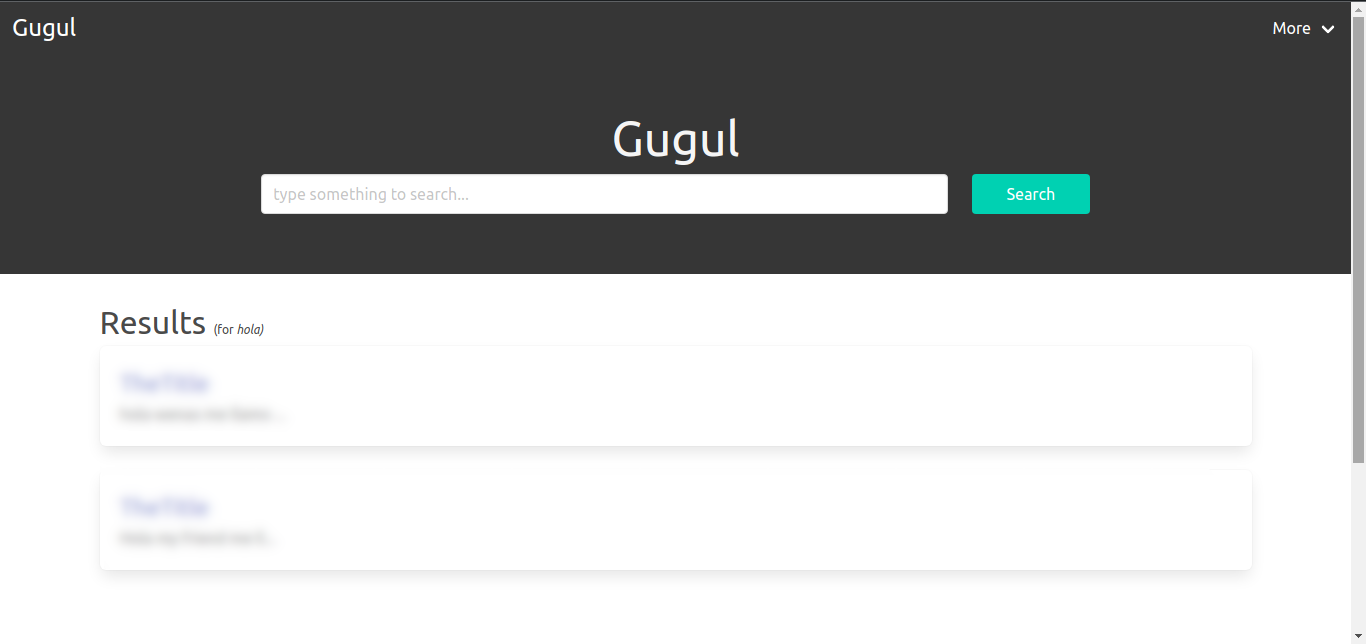
\includegraphics[width=0.5\linewidth]{img/pagprincipal.png} 
\end{center}


\paragraph{Historia}
Ruta:'/history' esta p\'agina muestra todos los t\'erminos que ha buscado el usuario, con hora y fecha , se guarda en la memoria interna del navagador, es decir una vez que se reinicie esta aplicaci\'on el historial estar\'a vac\'io de nuevo.

\begin{center}
	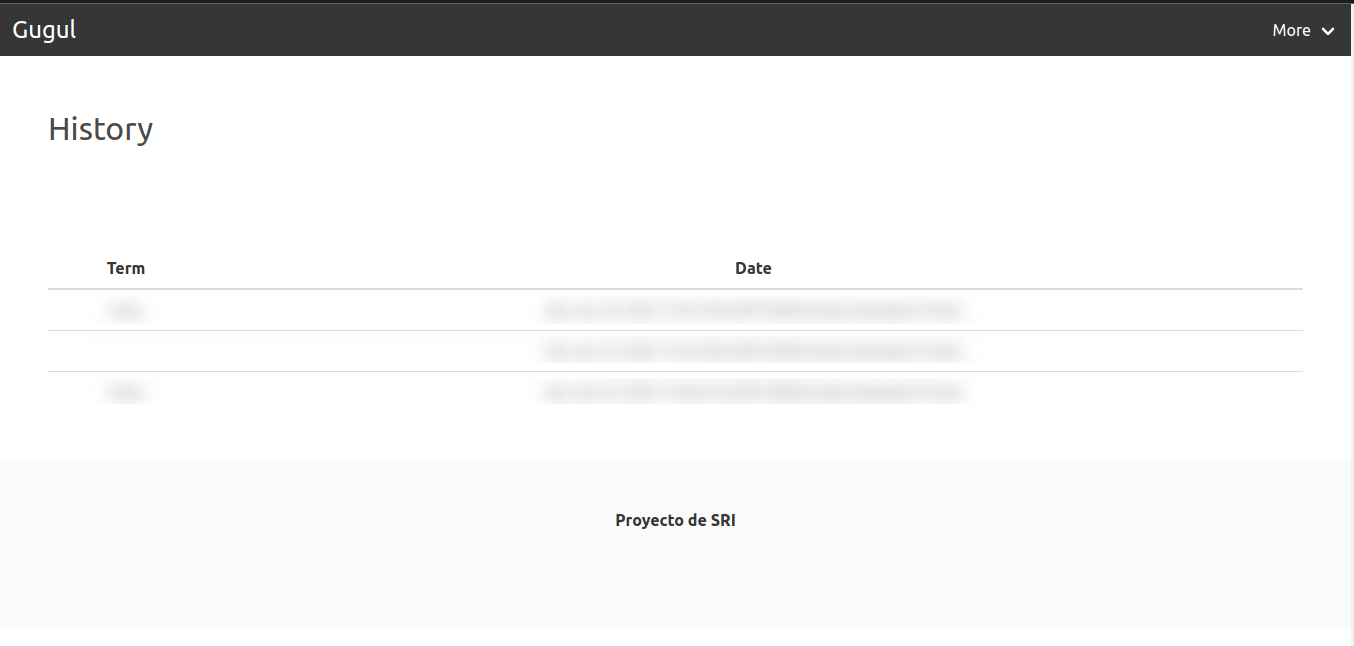
\includegraphics[width=0.5\linewidth]{img/history.png} 
\end{center}


\paragraph{Borrar historial}
Ruta:'/clear' en esta ruta se borra todo el hitorial que el usuario ha tenido desde que abri\'o el navegador

\begin{center}
	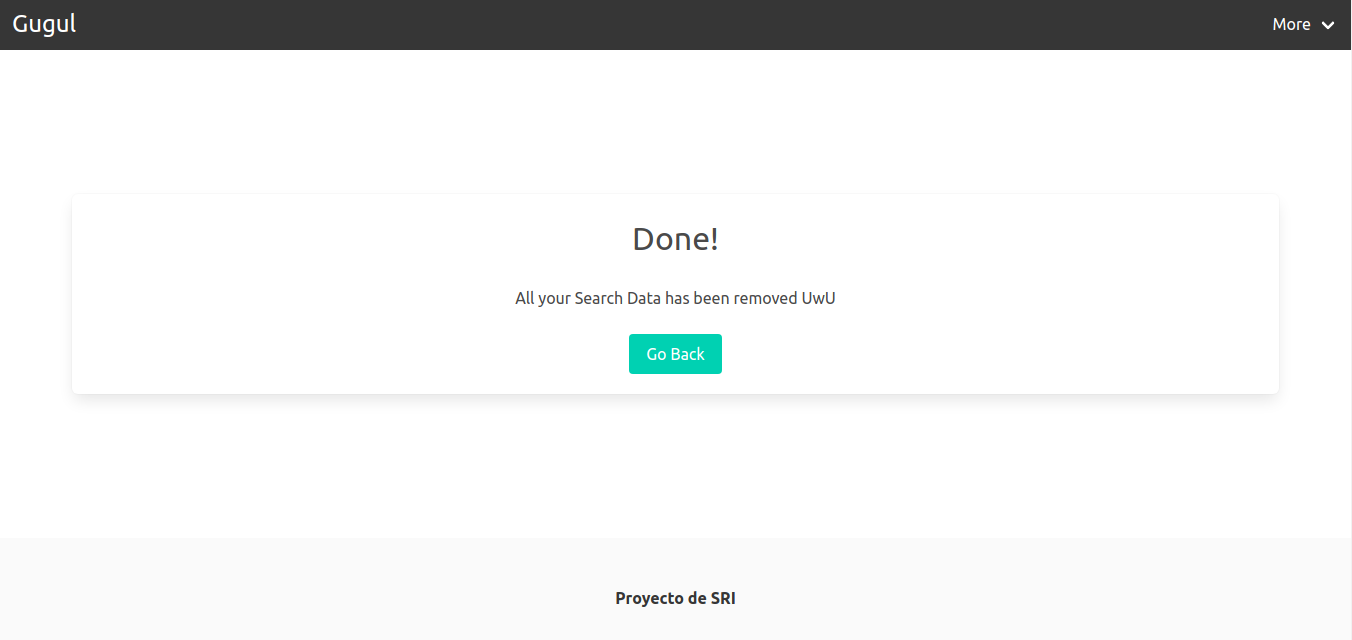
\includegraphics[width=0.5\linewidth]{img/clear.png} 
\end{center}

\paragraph{Banner}
Desde el banner de la p\'agina, en el botón desplegable More(esquina superior derecha), es posible acceder a la historia y a eliminar el historial, así como al precionar el nombre de la p\'agina en la esquina superior izquierda es posible acceder a la página principal.

\begin{center}
	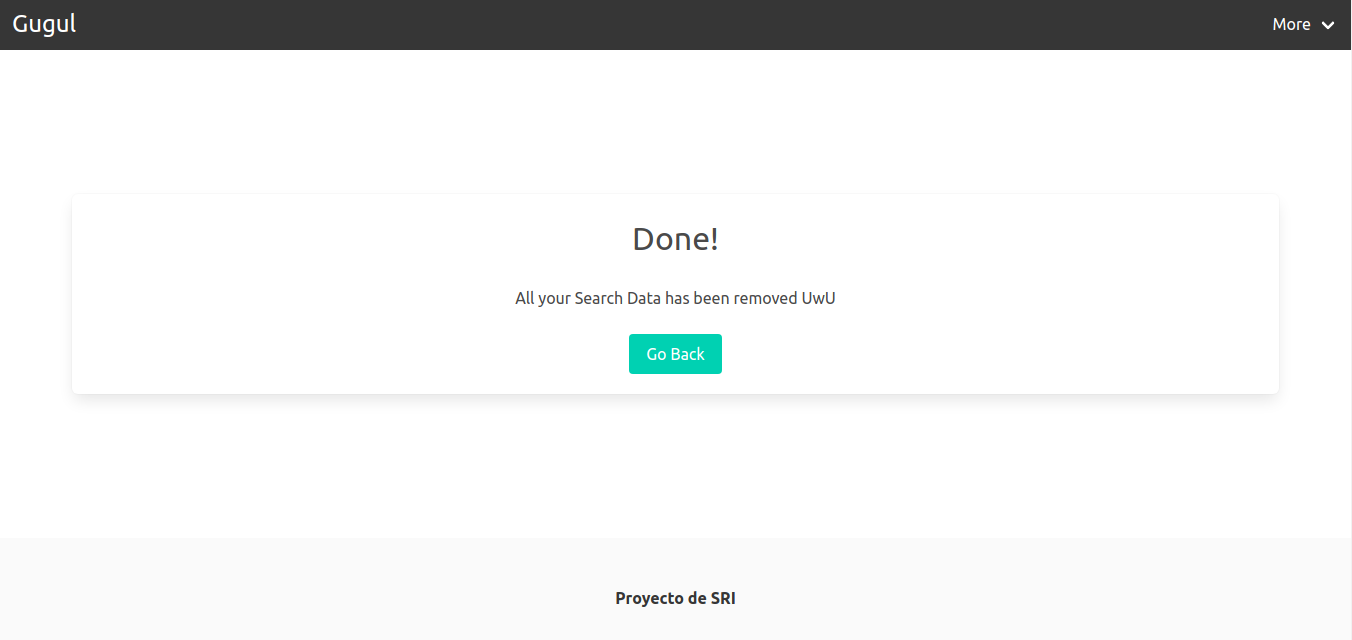
\includegraphics[width=0.5\linewidth]{img/clear.png} 
\end{center}

\section{An\'alisis cr\'itico de las ventajas y desventajas del sistema desarrollado.}


Se ha mostrado la arquitectura del modelo vectorial lo suficientemente abierto y flexible para ser usado en labores docentes, as\'i como investigaciones. La sencillez de esta arquitectura permitir\'a tanto la f\'acil observaci\'on de resultados y estructuras intermedias como la modificacion y a\~nadido de nuevos m\'odulos y por tanto permite experimentar con el modelo. Puede ser usado en la docencia de algunas materias relacionadas directamente con la extracci\'on automatizada de informaci\'on  


\paragraph{Ventajas}
Decidimos trabajar el modelo vectorial porque es un modelo que ha demostrado ser eficiente en SRI con repositorios grandes y de variadas tem\'aticas. En comparaci\'on con el modelo booleano es mejor para prop\'osito general, pues para booleano es recomendado que la informaci\'on que se trata de recolectar sea de un mismo tema, adem\'as de que es mas recomendable usar por expertos, no sucede asi con el vectorial, en cuyo caso puede ser usado facilmente por usuarios no expertos.

para el desarrollo del modelo usamos el esquema de ponderaci\'on \textit{tf-idf} pues para los documentos este esquema mejora el rendimiento de la recuperaci\'on. La estrategia de coincidencia parcial que usa el modelo permite la recuperaci\'on de los documentos que mas se aproximen a los requerimientos de la consulta. La estrategia permite ordenar los documentos por orden de similitud con la consulta.

\paragraph{Desventajas}
Un problema a resolver en el modelo es que  los t\'erminos indexados del documento son mutuamente independientes. Aunque en realidad existe relaci\'on entre algunos t\'erminos en el documento. Aunque podr\'ia significar una limitaci\'on del modelo simplifica el proceso de recuperaci\'on y en algunos casos mejora el rendimiento aunque a la hora de extracci\'on el proceso no sea tan abstracto como sistemas mas inteligantes. El an\'alisis de la correlacion requiere que se tangan enfoques mas avanzados en el sistema.

Este modelo necesita de la intersecci\'on de los t\'erminos de la consulta con los documentos, en caso contrario no se produce la recuperaci\'on de informaci\'on

Ademas al ser un modelo estad\'istico-matem\'atico, no tiene en cuenta la estructura sintáctico-semántica del lenguaje natural.

%
\section{Recomendaciones para trabajos futuros que mejoren la propuesta}

Para mejoras del sistema se propone al integraci\'on con algoritmos de `Crawling`. Adem\'as se puede trabajar en el reconocimiento de entidades que ayuden a una mejor vinculaci\'on entre diferenctes token de los documentos que guardan relaci\'on y pueden brindar mucha informaci\'on a la hora de determinar el peso de un documento en el \'ambito de la b\'usqueda . Tambi\'en se puede trabajar en correcciones b\'asicas como en interacciones con los usuarios que permitan al sistema saber que tan provechoso le fueron los resultado de la aplicaci\'on para una consulta dada, la informaci\'on recolectada se podr\'ia usar para pr\'oximas consultas similares o iguales.
%


\end{document}
